
\chapter{Verification of integration}
\label{cha:integration}

Figure~\ref{fig:scope-of-code-verification} on Page~\pageref{fig:scope-of-code-verification}
outlines the scope of code verification within OpenETCS.
Verification activities, however, also concern integration of the \isoc~code
with the \scade model (see Section~\ref{sec:integration-with-model})
and with the communication layers that underlies the bit stream abstractions
(see Section~\ref{sec:integration-with-communication}).

\section{Integration with \scade model}
\label{sec:integration-with-model}

The generated data packets from Chapter~\ref{cha:packets}
are sent and received over the so-called \emph{bit stream} layer
(see Chapter~\ref{cha:bitstream}).
In order to exchange the packets with the OpenETCS application
layer that is modeled in \scade (see Figure~\ref{fig:scope-of-code-verification})
the so-called \emph{integer stream} layer was defined.
Due to the relative late emergence of this layer in the OpenETCS project
this layer could not be formally be verified.
Rather it was tested together with underlying communication layer
(see Section~\ref{sec:integration-with-communication}).


\section{Integration with the underlying communication layer}
\label{sec:integration-with-communication}

The ETCS packets and messages which are decoded represent the bit
decoding and encoding layer as applied inside the
BTM and EURORADIO module as described inside\footnote{%
	See SUBSET-026, Chapter 2, Figure 1.
}.

Concerning the ETCS air gap messages it represents the layer for
bit encoding and decoding the ETCS content  
\begin{itemize}
\item \inl{coded_EUROBALISE_input_telegram}
\item \inl{coded_EURORADIO_output_msg} and
\item \inl{coded_EURORADIO_input_msg}
\end{itemize}

between the openETCS Kernel and the OpenETCS API (see Figure~\ref{fig:integration}).


The scope of the ETCS data packets is aligned with the openETCS show case
Amsterdam-Utrecht.
Thus not the complete set of packets can be decoded.
The supported packets are listed inside Section~\ref{sec:data-packets}.

\begin{figure}[hbt]
\begin{center}
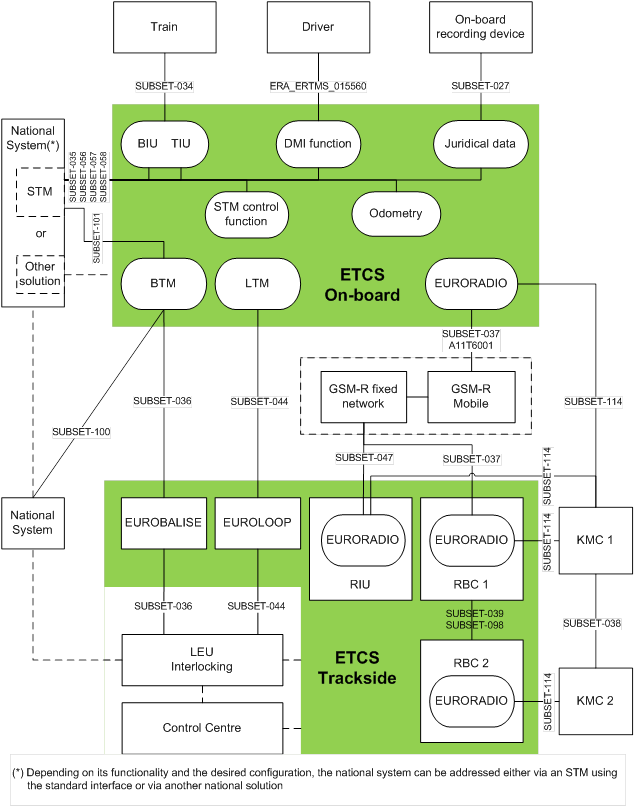
\includegraphics[width=0.99\textwidth]{figures/integration.png}
\caption{\label{fig:integration}
        Overview on integration interfaces.}
\end{center}
\end{figure}

\FloatBarrier
 
The OpenETCS decoder/encoder is referenced
as ``additional code components developed by other means''.\footnote{
	See Chapter 3.5 of Deliverable~2.3.
}.
It is generated from the requirement document of Subset-026-6
and SUBSET-026-7 to a XML model.
This model was verified manually against the SUBSET-026. 
Although not having a certified code generator the verification
is artifacts were verified after generation.


\clearpage

\section{Validation of the Implemented and Integrated Demonstration System}
\label{sec:VnV-Validation-DLR}


\paragraph{Contributing project partners}
The implementation and the validation of the integrated demonstration
system has been performed by the DLR with support of Fraunhofer FOKUS and
GE.


\paragraph{Process step}
This activity is part of the SW Validation (Phase~7). It contributes
to the Overall SW Test Report (7-29).


\paragraph{Object of validation}
The integrated demonstration system is validated. It consists of 2
basic subsystems: the EVC and the DMI. The implementations of both
subsystems are generated from the according operators of the SCADE
model using the Esterel code generator KCG. The complete integrated
demonstration system includes the target platforms and communication
systems as well. The triggering of the EVC as well as of the DMI needs
to be realised by a platform dependent wrapper. This wrapper has also
to handle the communication channels and resources. The wrapper for
EVC and DMI depend completely on the chosen target platform and are
implemented manually. However, the basic structure and basic schemes
are identical since both wrappers have the same tasks.


\paragraph{Available specification}
The modelled SCADE simulation of the EVC and DMI running from
Amsterdam to Utrecht is used as behavioural reference
specification. All driver relevant outputs - such as speeds,
distances, and state changes - are relevant for the validation.


\paragraph{Objective}
Basic assumption for model driven code generation is the correctness
of the code generator. This assumption is also stated for the
KCG-generated model code. Hence, the functionality of the implemented
EVC and the implemented DMI is not verified, since the verification is
already done on model level.

Furthermore, the interaction of each subsystem on a physical hardware
platform needs to be validated for correct functional
behaviour. Especially platform related resource restrictions or timing
issues may influence the overall behaviour of the generated
implementations of the subsystems.


\paragraph{Method/Approach}
The validation is realised by running the test track (Amsterdam -
Utrecht). A concrete sequence of activities is defined in order to
start-up and initiate the distributed system. External inputs,
e.g. for TIU, odometry, and balise information, are provided by a
simulation platform (SEFEV, proprietary software for executing
Subset076 sequences) which is connected via TCP-sockets to the
EVC. The behaviour of the integrated demonstration system is compared
to the behaviour of the SCADE-simulation model. Tolerances for time
and distances have been used as specified in Subset076.

The log files of each subsystem were used in order to check concrete behaviour.


\paragraph{Results}
The validation was done based on Win32-implementations of each
subsystem (EVC, DMI). Both subsystems were executed as single
processes on the same machine. The communication was realised via
TCP-sockets. The correct behaviour of the implementation compared to
the simulated model was shown for a first part of the test drive of
around 4km.


\paragraph{Observations/Comments}
A second implementation of the demonstrations system was realised on
an embedded real-time platform. The EVC was executed on this platform
whereas the DMI needed to be executed on a Win32-platform. The
generated code for EVC and DMI were identical to the code of the
initial Win32-implementation. Only the platform dependent wrappers and
the communication management needed to be adopted.

Due to timing and resource restrictions of the real-time platform,
several synchronization issues needed to be solved. It can be stated
that the execution times of each part of the subsystem may influence
the overall functional behavior.


\paragraph{Conclusion}
The generated implementation of the SCADE model and the basic wrapping
systems work as expected. Further investigations are necessary in
order to validate runtime and synchronization effects - mainly on
heterogeneous target platforms.
